\chapter{Implementação e Resultados}
\label{chapter:implementacaoResultados}
\noindent
Neste trabalho, foram empregados dois modelos de representação de textos distintos. Cada modelo foi utilizado para gerar um descritor por questão com base no enunciado e alternativas. Esses descritores juntos aos rótulos de disciplina serviram de fonte de dados para modelos classificadores os quais foram comparados pela sua acurácia.

Para estabelecer um padrão de comparação entre os distintos modelos, definiu-se um conjunto de parâmetros da API de dados descrita na seção \ref{dataset_api}. Dentre esses parâmetros, pode-se destacar o uso de um dicionário de agrupamento de assuntos conforme listado no apêndice \ref{JSON_dict} e um número mínimo de 10000 amostras por categoria de enunciado. A partir desses parâmetros, as 133 classes iniciais listadas no apêndice \ref{questoes_lista} foram reduzidas a apenas 9 classes conforme ilustra a figura \ref{fig:pie_labels_graph}.

\begin{figure}[!ht]
	\centering
	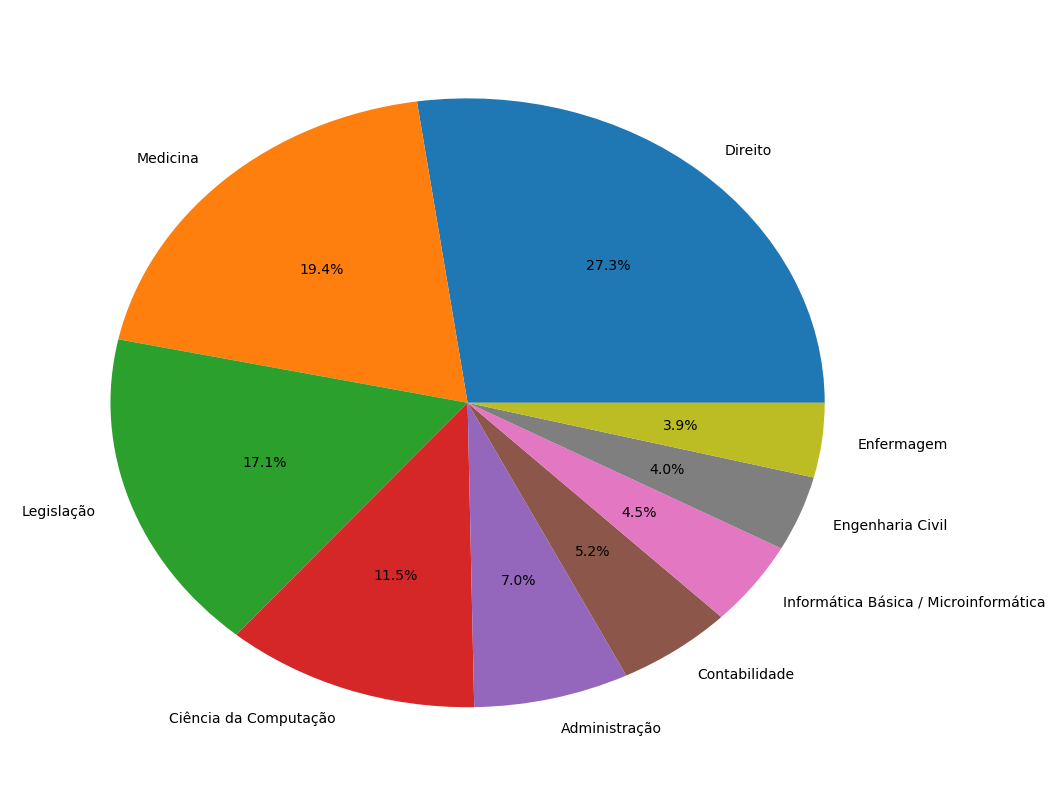
\includegraphics[width=1.0\textwidth]{figures/pie_graph.png}
	\caption{Distribuição das categorias selecionadas}
	\label{fig:pie_labels_graph}
\end{figure}

\section{\textit{Bag of words}} \label{bow_implementation}

Para a representação \textit{bag of words}, foram utilizados algoritmos classificadores tradicionais conforme descrito em \cite{InformationRetrievalBook}. Como algoritmos populares, eles atuam como uma referência de \textit{benchmarking} para os modelos mais modernos que serão discutidos na seção \ref{We_implementation}.

Como etapas de preparação da estrutura de dados a partir da representação \textit{bag of words}, foram utilizadas as seguintes técnicas de processamento de linguagem natural do pacote NLTK (\textit{Natural Language Toolkit}), que possui suporte para a linguagem português brasileiro: a separação da frase em palavras, deixando-as com letra minúscula; a remoção de \textit{stopwords} (palavras de parada) desse conjunto de palavras, apresentadas no apêndice \ref{stopwords}; e a lematização das palavras utilizando \textit{RSLPStemmer} (Removedor de Sufixos da Língua Portuguesa) (\cite{RSLPStemmer}). Após a aplicação dessas técnicas, é utilizado TF-IDF por meio da implementação \textit{TfidfTransformer} da biblioteca \textit{scikit-learn}.

\subsection{\textit{Naive Bayes}}

\textit{Naive Bayes} é um algoritmo de classificação baseado no teorema de Bayes de probabilidade e a versão utilizada nessa implementação foi a variante multinomial que, como o próprio sugere, assume uma distribuição multinomial na inferência de probabilidade. Este classificador é popular para classificações discretas, como é o caso da classificação de textos conforme já explorado por \cite{McCallum98acomparison}.

Utilizou-se a implementação da biblioteca do \textit{sklearn}, obtendo-se resultados sumarizados pela figura \ref{fig:confusion_matrix_NB} e pela tabela \ref{tab:NB}.

\begin{table}[ht]
\centering
\caption{Métricas do modelo \textit{naive bayes}}
\vspace{0.5cm}
\begin{tabular}{c|c|c}
 
Métrica & Conj. de Treinamento & Conj. de Teste \\
\hline
Acurácia & 0.79287 & 0.78655 \\
F1-Score & 0.77180 & 0.76427 \\
Precisão & 0.80543 & 0.79806 \\
AUC ROC  & 0.97163 & 0.96980
\end{tabular}
\label{tab:NB}
\end{table}

\begin{figure}[!ht]
	\centering
	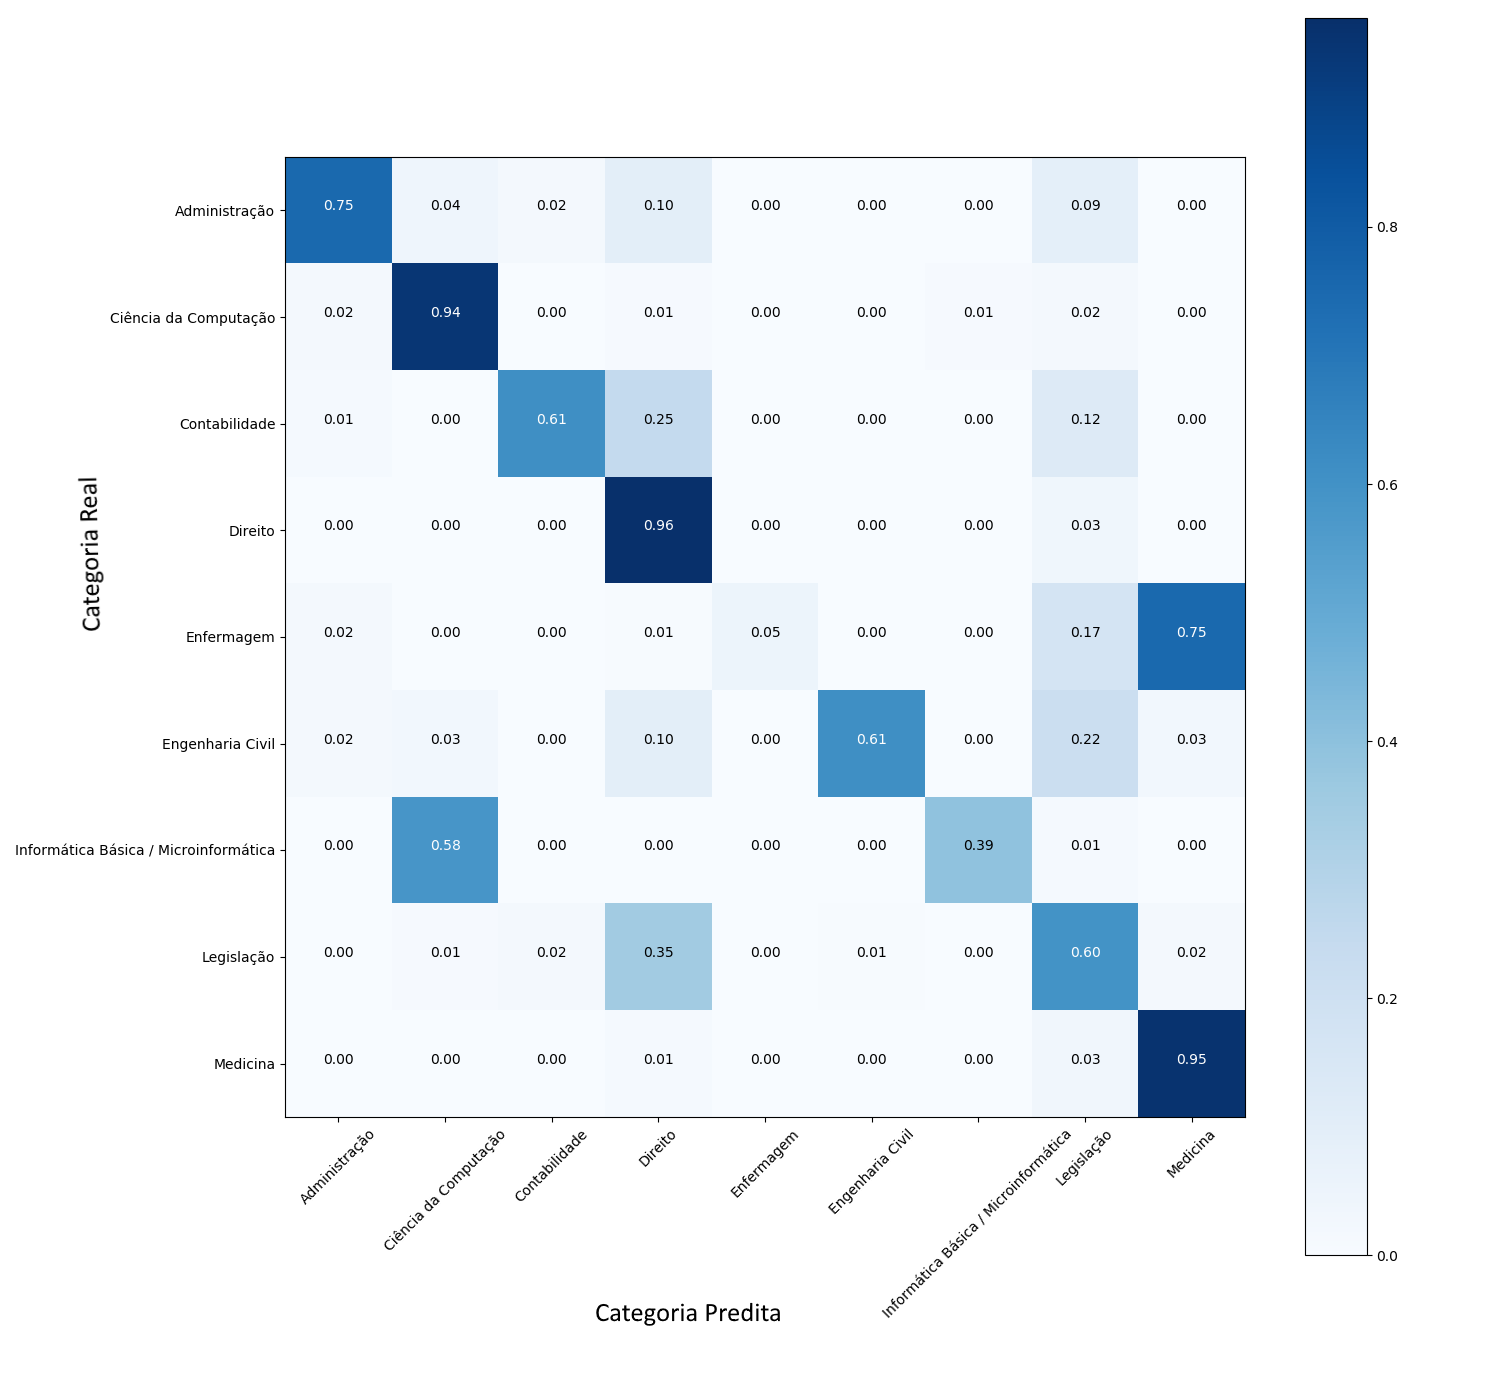
\includegraphics[width=1.1\textwidth]{figures/NB_-_Confusion_matrix_normalized_-_test.png}
	\caption{Matriz de confusão no conjunto de testes para o classificador Naive Bayes}
	\label{fig:confusion_matrix_NB}
\end{figure}

\subsection{\textit{Support Vector Machines}}

Conforme descrito por \cite{SVM4textClassification}, \textit{Support Vector Machines} é um algoritmo de aprendizado de máquina que se destaca na classificação de textos devido à sua robustez ao lidar com dados de entrada de alta dimensionalidade e esparsos como é o caso dos dados gerados a partir da representação \textit{bag of words}.

A implementação escolhida para esse classificador foi também a da biblioteca \textit{sklearn} a partir do método \textit{SGDClassifier}, resultando na matriz de confusão da figura \ref{fig:confusion_matrix_SVM} em que as métricas são detalhadas pela tabela \ref{tab:SVM}.

\begin{table}[ht]
\centering
\caption{Métricas do modelo \textit{SVM}}
\vspace{0.5cm}
\begin{tabular}{c|c|c}
 
Métrica & Conj. de Treinamento & Conj. de Teste \\
\hline
Acurácia & 0.77368 & 0.77295 \\
F1-Score & 0.74712 & 0.74489 \\
Precisão & 0.78709 & 0.78676
\end{tabular}
\label{tab:SVM}
\end{table}

\begin{figure}[!ht]
	\centering
	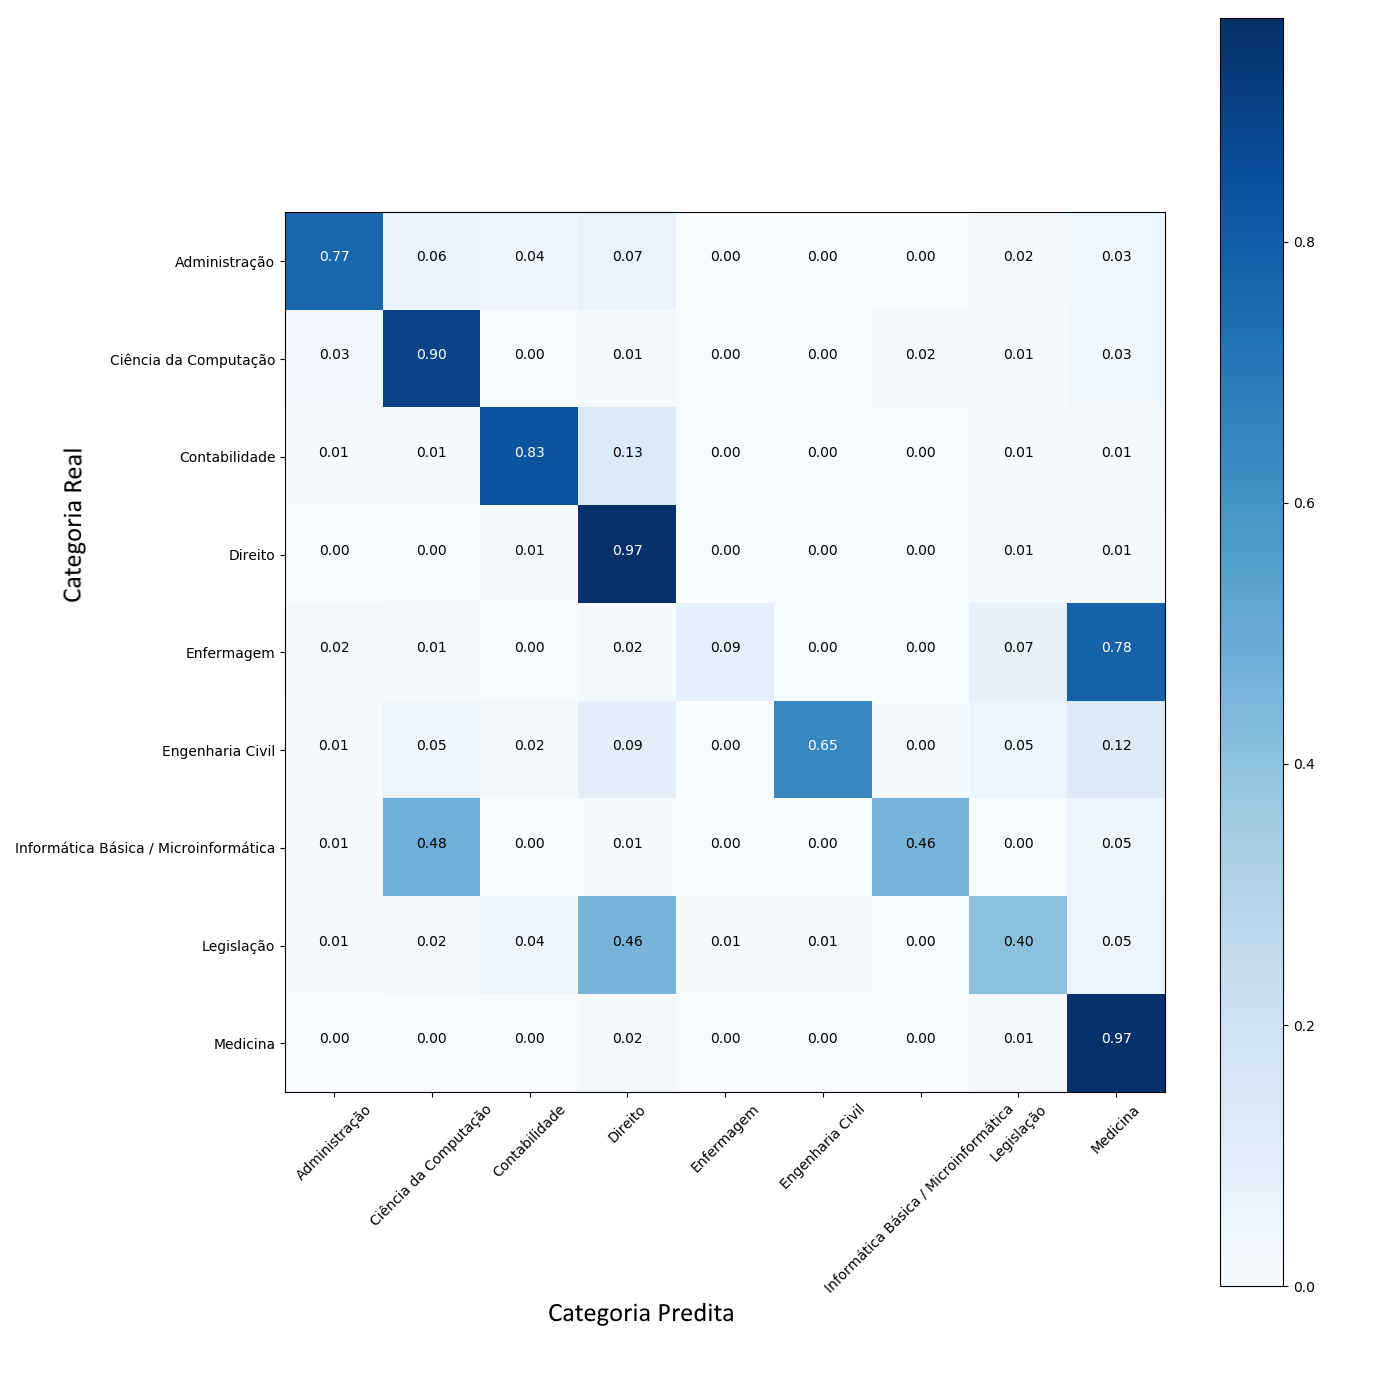
\includegraphics[width=1.1\textwidth]{figures/SVM_Confusion_matrix_normalized.png}
	\caption{Matriz de confusão no conjunto de testes para o classificador SVM}
	\label{fig:confusion_matrix_SVM}
\end{figure}

\section{Word embedding} \label{We_implementation}
Foram utilizados vetores gerados por meio da técnica GloVe \citep{pennington2014glove} que foram treinados em língua portuguesa e disponibilizados pelo NILC-USP \citep{DBLP:journals/corr/Ruder16}. A implementação foi realizada com vetores de 50, 100, 300, 600 e 1000 dimensões.

\subsection{Média simples}
Junto ao modelo de word embedding, utilizou-se uma regressão logística conforme a figura \ref{fig:simple_avg} onde cada entrada $V$ de $N$ dimensões corresponde a média aritmética das palavras no enunciado $S$ da respectiva questão, ou seja:

\begin{figure}[!ht]
	\centering
	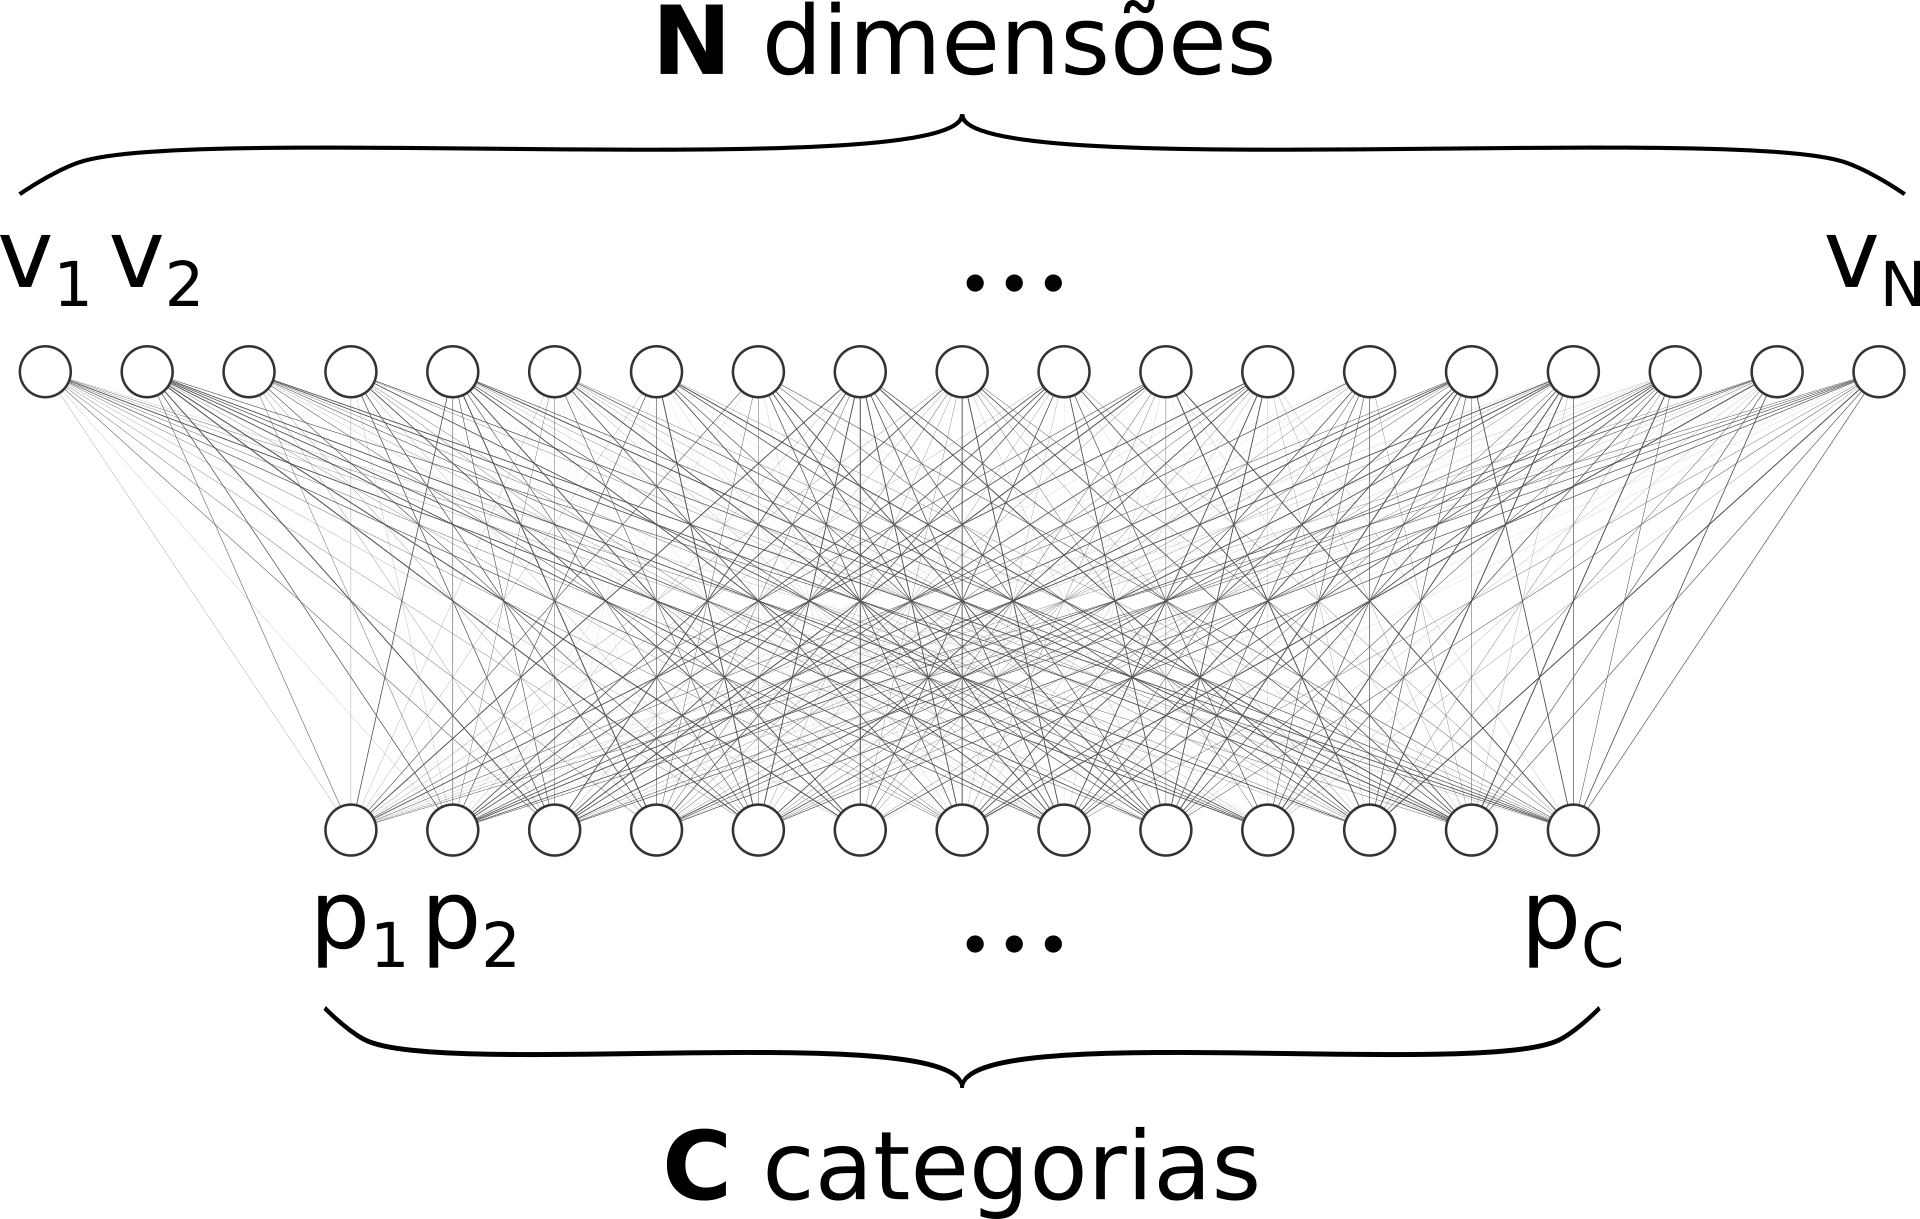
\includegraphics[width=0.6\textwidth]{figures/simple_avg.png}
	\caption{Média simples}
	\label{fig:simple_avg}
\end{figure}

$$v_i = \dfrac {\sum_{w \in S} \text{glove}(w)} {L_S}$$

Onde $v_i$ é o i-ésimo valor de entrada para a rede em que $i \in [1,N]$ e $S = \{w_1, w_2, \cdots\}$ é a sequência das $L_S$ palavras $w$ no enunciado $S$.

A implementação utilizou a linguagem Python e a biblioteca de aprendizado de máquinas Tensorflow, produzindo os resultados indicados na tabela \ref{tab:simple_avg}.

\begin{table}[ht]
\centering
\caption{Métricas do modelo no conjunto de testes para os distintos números de dimensões de  \textit{word embedding} analisados}
\vspace{0.5cm}
\begin{tabular}{c|c|c|c|c}
 
Dimensões & Acurácia & F1-Score & Precisão & AUC ROC\\
\hline
50   & 0.7368 & 0.7213 & 0.7239 & 0.9497\\
100  & 0.7641 & 0.7552 & 0.7551 & 0.9583\\
300  & 0.8014 & 0.7940 & 0.7949 & 0.9689\\
600  & 0.8146 & 0.8082 & 0.8094 & 0.9724\\
1000 & 0.8216 & 0.8171 & 0.8183 & 0.9746
\end{tabular}
\label{tab:simple_avg}
\end{table}

Apesar de ser um modelo simples, um ponto de destaque foi a sua capacidade de generalização. Não foi observada tendência de \textit{overfitting} conforme ilustra o gráfico da figura \ref{fig:loss_50}.

\begin{figure}[!ht]
	\centering
	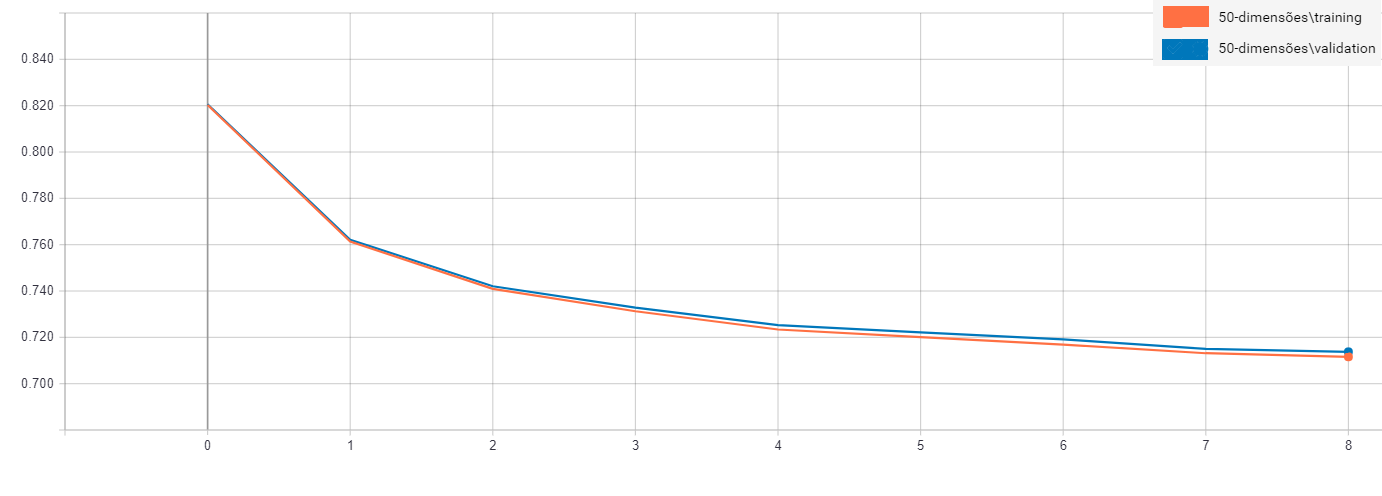
\includegraphics[width=1.1\textwidth]{figures/loss-50.PNG}
	\caption{Curva da função de custo ao término de cada epoch de treinamento para 50 dimensões de \textit{word embedding}}
	\label{fig:loss_50}
\end{figure}

Além disso, como era de se esperar a partir dos resultados listados na tabela \ref{tab:simple_avg}, houve uma boa separação das classes selecionadas nas previsões. Conforme apresenta a figura \ref{fig:confusion_matrix_1000_simpleAvg}, apenas categorias que são difíceis de serem distinguidas até mesmo por seres humanos tiveram um índice de acerto menor do que 83\%. Nesses casos, as classes majoritárias, vide figura \ref{fig:pie_labels_graph}, foram favorecidas.

\begin{figure}[!ht]
	\centering
	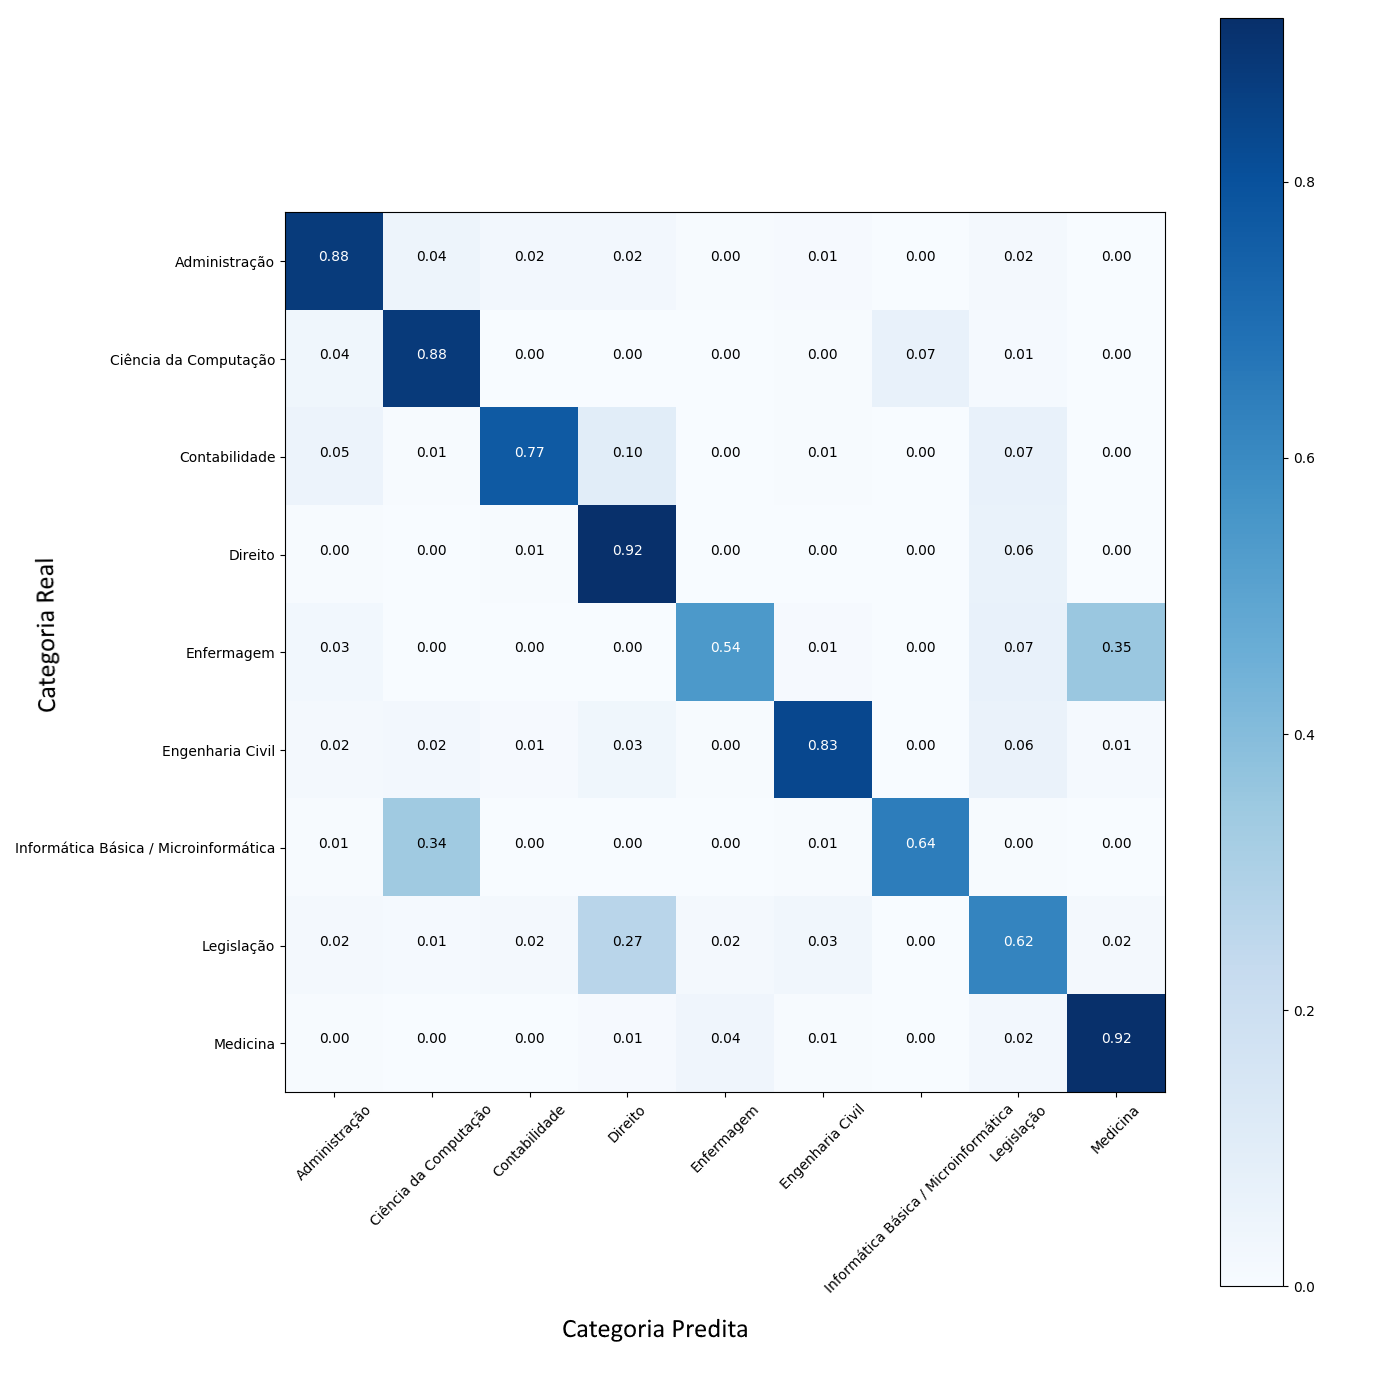
\includegraphics[width=1.1\textwidth]{figures/SimpleAvg_1000_Confusion_matrixnormalized.png}
	\caption{Matriz de confusão no conjunto de testes com o uso de 1000 dimensões de \textit{word embedding}}
	\label{fig:confusion_matrix_1000_simpleAvg}
\end{figure}

\section{Arquitetura }

Nas implementações de classificadores descritas nas seções \ref{bow_implementation} e \ref{We_implementation}, existem várias etapas em comum. Em virtude disso, buscou-se realizar uma implementação que satisfizesse requisitos de manutenibilidade e reusabilidade. Dessa forma, foi elaborada uma solução focada em uma hierarquia de classes que maximizasse o reúso de implementações entre os modelos conforme ilustra o diagrama de classes na figura \ref{fig:ClassDiagram}. Parte-se de uma classe abstrata (BaseModel) que define a interface básica e implementa métodos relacionados a exibição de resultados e a admissão de dados. Essa classe é então especializada de acordo com as duas estruturas de dados para a representação de texto em concordância com as definições do capítulo \ref{cap:methods}. Por fim, especializa-se de acordo com o algoritmo classificador utilizado, podendo haver ainda uma especialização seguinte para diferentes topologias do classificador em questão.

\begin{figure}[!ht]
	\centering
	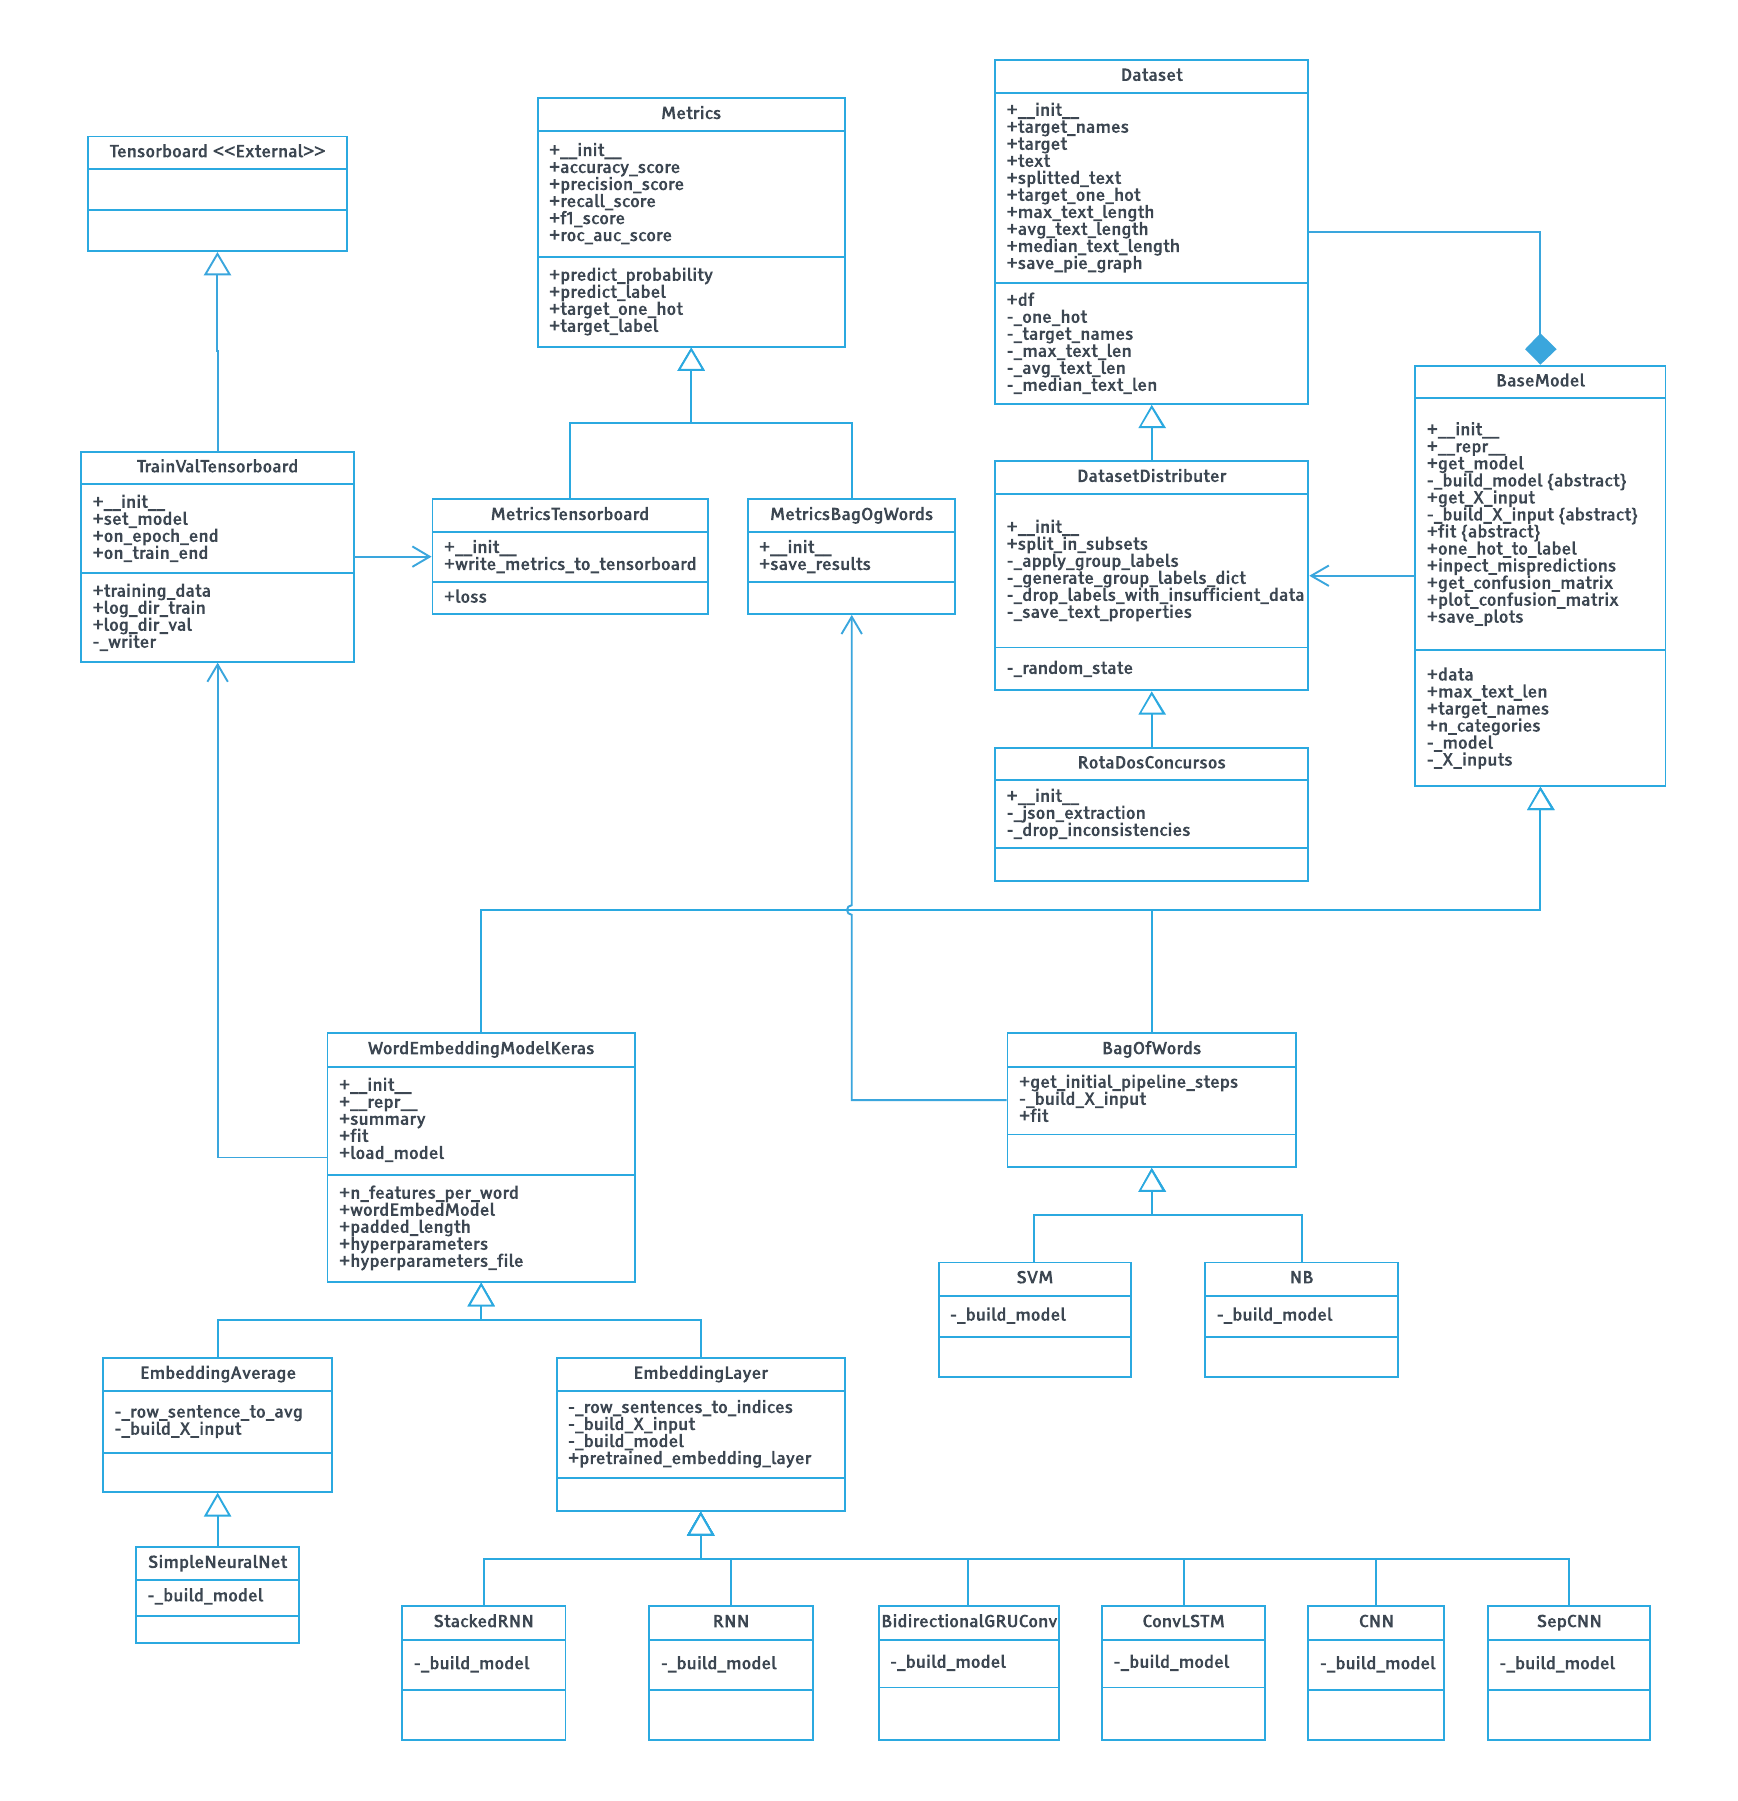
\includegraphics[width=1.18\textwidth]{figures/ClassDiagram.png}
	\caption{Diagrama de classes}
	\label{fig:ClassDiagram}
\end{figure}

Um aspecto da implementação que foi de grande importância na viabilização da execução dos treinamentos foi a facilidade de se utilizar vários núcleos de processamento ao utilizar bibliotecas como scikit-learn e keras/tensorflow. Isso permitiu a paralelização utilizando vários núcleos de um servidor robusto do serviço AWS da Amazon conforme ilustra a figura \ref{fig:paralelization_AWS}.

\begin{figure}[!ht]
	\centering
	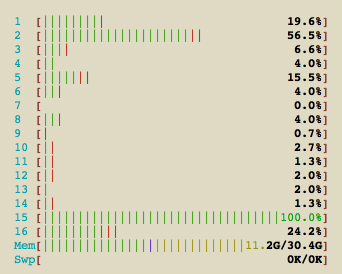
\includegraphics[width=0.6\textwidth]{figures/htop.png}
	\caption{Uso das CPUs no servidor durante um dos treinamentos}
	\label{fig:paralelization_AWS}
\end{figure}

Por fim, visando a rastreabilidade das alterações do código durante o desenvolvimento e uma colaboração em equipe, todo o código foi versionado. O repositório pode ser acessado em: github.com/brunovcosta/pfc .